

\section{S.T.A.N.R.I}

\begin{center}
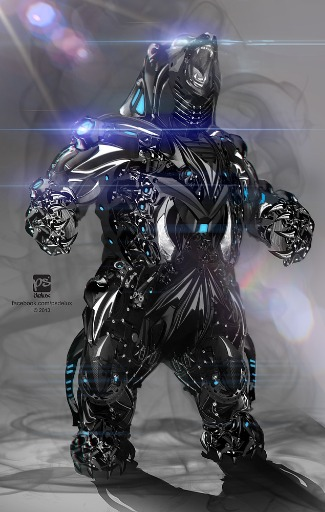
\includegraphics[width=80mm]{./content/img/stanriMecha.jpg}
\begin{figure}[h]
\end{figure}
\end{center}


\subsubsection{Background}

S.T.A.N.R.I was created by Exme as a battle companion.  S.T.A.N.R.I originally used a human brain as a counter balance which resulted in a large amount of leaking.    

S.T.A.N.R.I started off life as a small robo-cub called Stanri Mk 0, as Exme continued to develop her plans for what he would finally become.  Baby Stanri was a small, loveable robot with a tendency to leak (this was due to the ongoing putrification of a human brain that had been placed inside Stanri under the mistaken idea that it would act as a balancing measure).  

During the siege of Ruh'Breks tower, the workshop managed to complete the constructions of S.T.A.N.R.I Mk I and dispatched it immediately through a teleporter.  Stanri's brain unit was revelaed to be a battle computer that had been collecting battle and movement data for months now.  This was transferred into S.T.A.N.R.I and functioned as its main CPU.   

\subsubsection{Functions}

Stanri Mk 0 had limited functionality and little to no battle capability.  He could respond to basic commands and carry a limited amount of weight.     

S.T.A.N.R.I Mk I was a fully operational combat unit that was able to enter battle, following commands of his master Exmerah, as well as other team members.  S.T.A.N.R.I was able to make attacks using his two powerful claws and devastating bite attack.  In addition to his usefulness as a battle companion, S.T.A.N.R.I  was able to offer a range of additional analytical capabilities, including an improved ofalcatory sensing unit, on-board item analysis and communications with the airship.  

During the Linderdorf campaign, Exme provided plans to the Gnomes XXX who managed to convert S.T.A.N.R.I into his final form.  Taking on the shape of a tiger in honour of their former companion Mr Tiger, and making use of the new access to Excallibrum, Exme and the Gnomes were able to enhance S.T.A.N.R.I's functionality and turn him into a battlesuit for Exme.  In his so=called `Mecha-form' Exme was able to wear S.T.A.N.R.I as a suit of armour, with his onboard power generators providing enhancements to C.E.D.R.I.C to increase their firepower significantly.

Following the release of The Seven, S.T.A.N.R.I was gifted conciousness as a reward for his efforts in bringing back the Gods to the world.  

\begin{center}
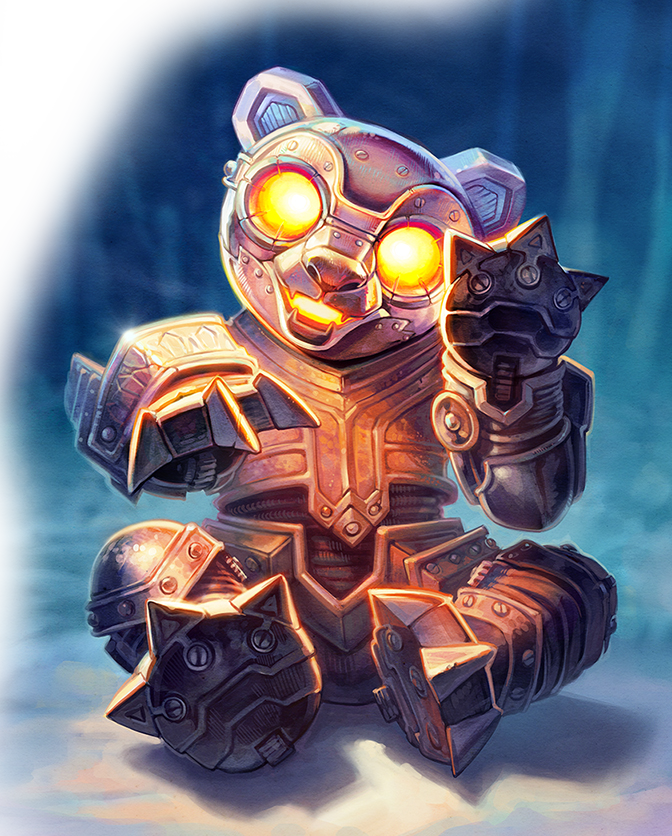
\includegraphics[width=80mm]{./content/img/babyStanri.png}
\begin{figure}[h]
\end{figure}
\end{center}


\clearpage